\documentclass[11pt]{article}

\usepackage[landscape,margin=0.6in]{geometry}
\usepackage{amsmath,amssymb}
\usepackage{tikz}
\usepackage{xcolor}
\usepackage{microtype}

\usetikzlibrary{arrows.meta,positioning,calc,patterns}

\newcommand{\dd}{\mathrm d}
\newcommand{\1}{\mathbf 1}

\definecolor{ink}{RGB}{35,35,35}
\definecolor{accent}{RGB}{38,98,135}
\definecolor{muted}{RGB}{105,105,105}
\definecolor{softblue}{RGB}{231,242,248}
\definecolor{softgreen}{RGB}{232,244,236}
\definecolor{softred}{RGB}{249,235,232}

\pagestyle{empty}

\tikzset{
  axis/.style={->,thick,draw=ink},
  curve/.style={very thick,draw=accent},
  arrow/.style={-{Latex[length=3mm]},thick,draw=accent},
  redarrow/.style={-{Latex[length=3mm]},thick,draw=red!65!black},
  note/.style={font=\small,align=center,text=ink},
  smallnote/.style={font=\scriptsize,align=center,text=muted},
  box/.style={draw=ink,rounded corners=2pt,thick,align=center,inner sep=7pt,minimum height=1.0cm,fill=white},
  bluebox/.style={box,fill=softblue},
  greenbox/.style={box,fill=softgreen},
  redbox/.style={box,fill=softred}
}

\begin{document}

\begin{center}
{\Large Figure 1. Fertility Response to a Binding Family-Housing Cap}
\end{center}

\vspace{0.3cm}

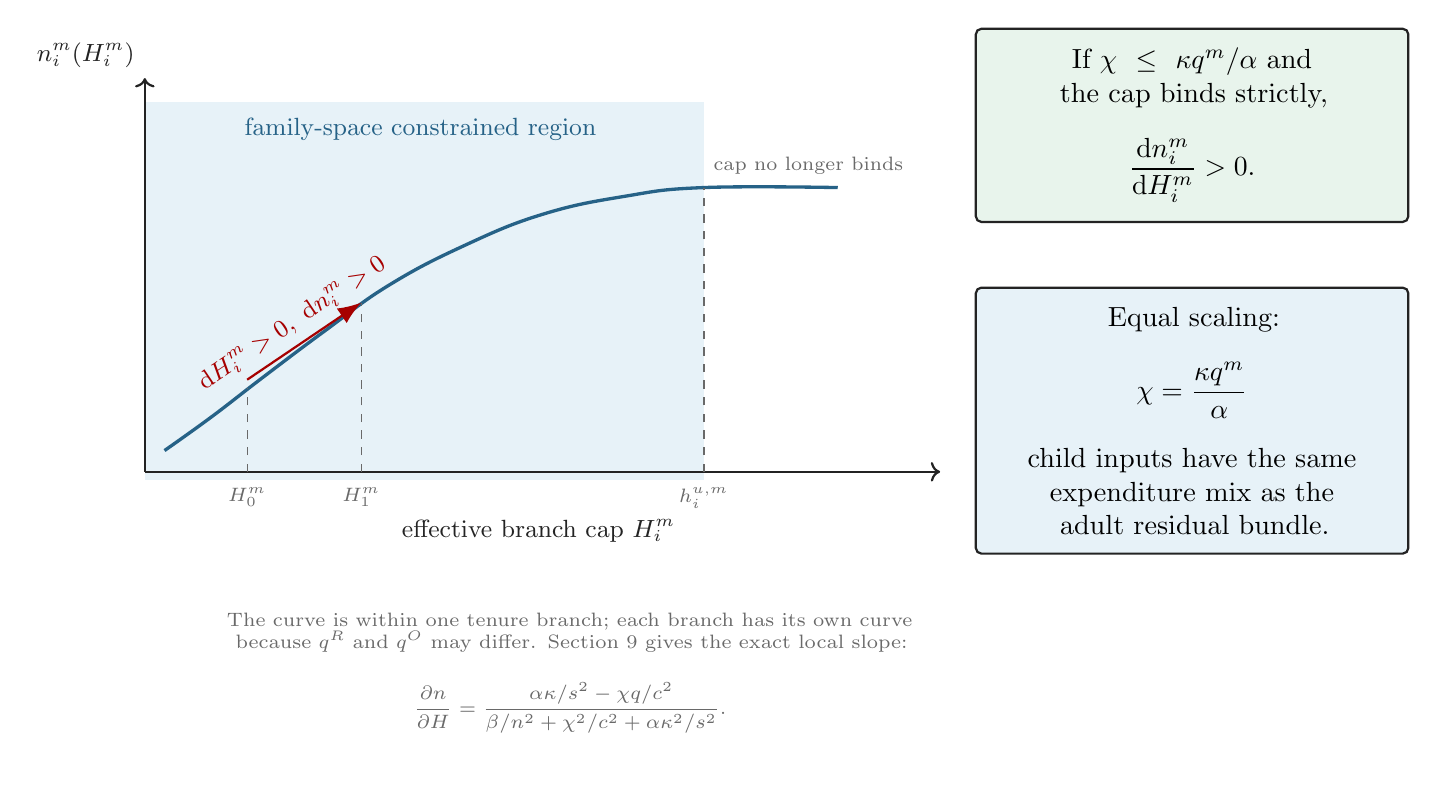
\begin{tikzpicture}[x=1cm,y=1cm]
  \fill[softblue] (0.7,0.45) rectangle (7.8,5.25);
  \node[note,text=accent] at (4.2,4.9) {family-space constrained region};

  \draw[axis] (0.7,0.55) -- (10.8,0.55);
  \node[note] at (5.7,-0.2) {effective branch cap $H_i^m$};
  \draw[axis] (0.7,0.55) -- (0.7,5.55) node[above left,note] {$n_i^m(H_i^m)$};

  \draw[curve]
    plot[smooth,tension=0.72] coordinates {
      (0.95,0.82) (1.55,1.25) (2.2,1.75) (3.0,2.35)
      (3.8,2.92) (4.75,3.42) (5.75,3.82) (6.8,4.05)
      (7.8,4.16) (9.5,4.16)
    };

  \draw[dashed,thick,draw=muted] (7.8,0.55) -- (7.8,4.16);
  \node[smallnote,below] at (7.8,0.48) {$h_i^{u,m}$};
  \node[smallnote,above right] at (7.8,4.2) {cap no longer binds};

  \draw[dashed,draw=muted] (2.0,0.55) -- (2.0,1.62);
  \node[smallnote,below] at (2.0,0.48) {$H_0^m$};
  \draw[dashed,draw=muted] (3.45,0.55) -- (3.45,2.7);
  \node[smallnote,below] at (3.45,0.48) {$H_1^m$};

  \draw[redarrow] (2.0,1.72) -- (3.45,2.7)
    node[midway,above,sloped,note,text=red!65!black] {$\dd H_i^m>0,\ \dd n_i^m>0$};

  \node[bluebox,text width=5.0cm] at (14.0,1.20) {
    Equal scaling:
    \[
      \chi=\frac{\kappa q^m}{\alpha}
    \]
    child inputs have the same expenditure mix as the adult residual bundle.
  };

  \node[greenbox,text width=5.0cm] at (14.0,4.95) {
    If $\chi\le \kappa q^m/\alpha$ and the cap binds strictly,
    \[
      \frac{\dd n_i^m}{\dd H_i^m}>0.
    \]
  };

  \node[smallnote,text width=12.0cm] at (6.1,-2.2) {
    The curve is within one tenure branch; each branch has its own curve because $q^R$ and $q^O$ may differ. Section 9 gives the exact local slope:
    \[
    \frac{\partial n}{\partial H}
    =
    \frac{\alpha\kappa/s^2-\chi q/c^2}
    {\beta/n^2+\chi^2/c^2+\alpha\kappa^2/s^2}.
    \]
  };
\end{tikzpicture}

\clearpage

\begin{center}
{\Large Figure 2. A Local Policy Decomposition for Fertility Effects}
\end{center}

\vspace{0.2cm}

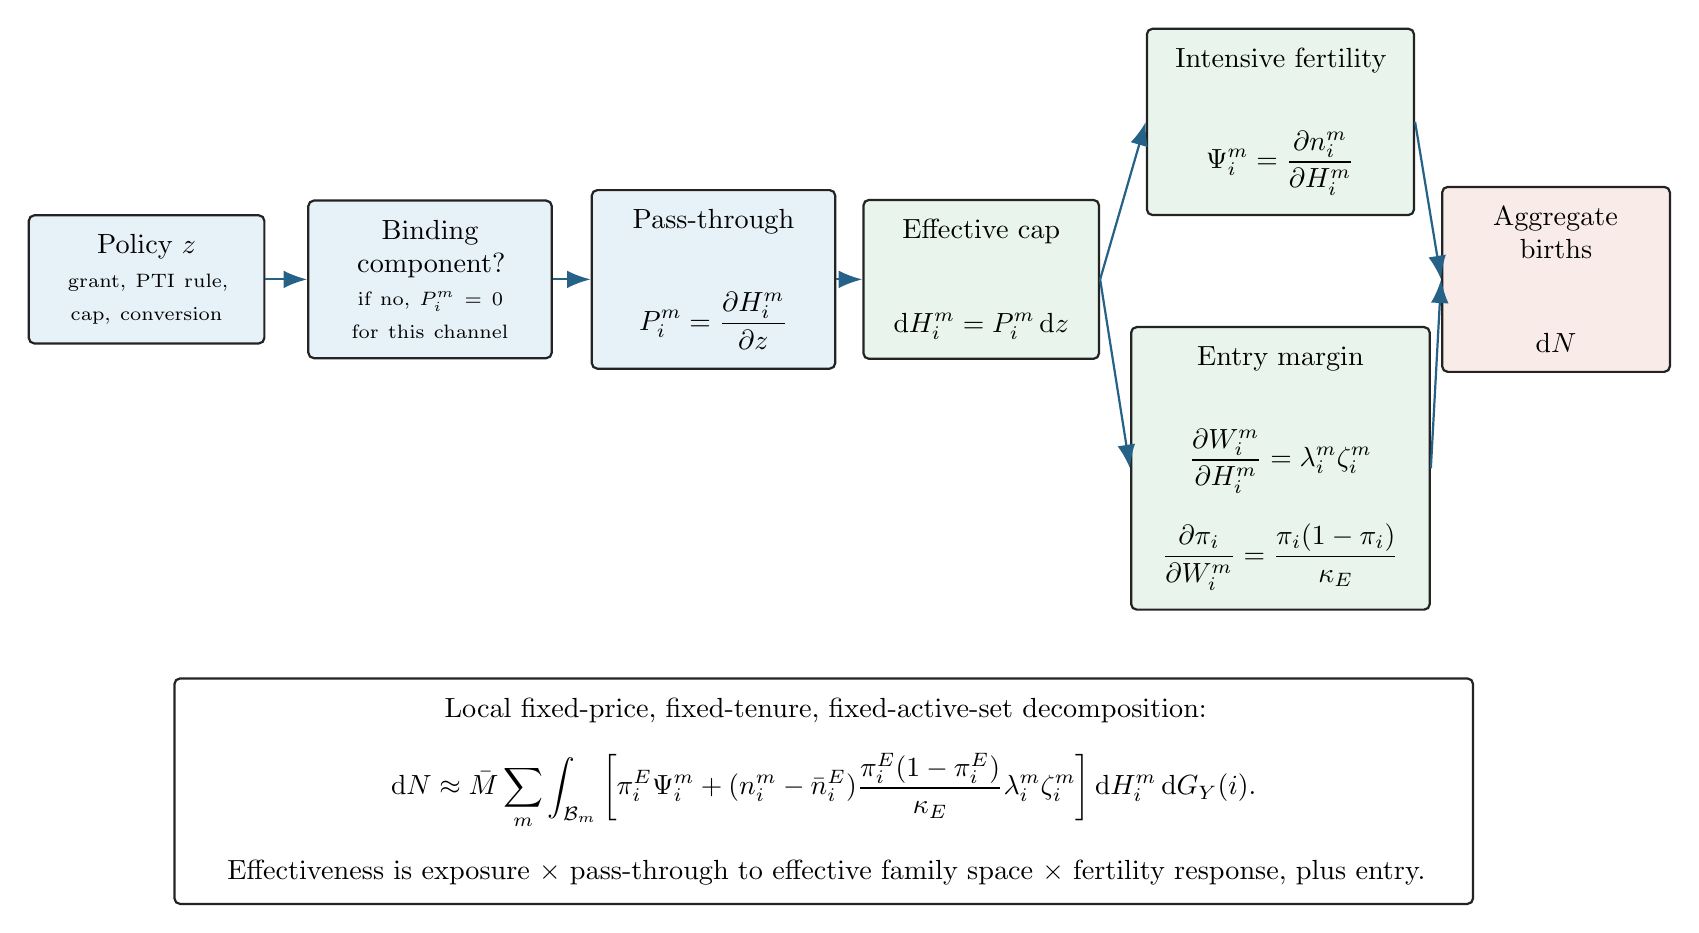
\begin{tikzpicture}[x=1cm,y=1cm]
  \node[bluebox,text width=2.5cm] (policy) at (0,1.6) {
    Policy $z$\\
    \scriptsize grant, PTI rule, cap, conversion
  };
  \node[bluebox,text width=2.6cm] (gate) at (3.6,1.6) {
    Binding component?\\
    \scriptsize if no, $P_i^m=0$ for this channel
  };
  \node[bluebox,text width=2.6cm] (pass) at (7.2,1.6) {
    Pass-through\\
    \[
      P_i^m=\frac{\partial H_i^m}{\partial z}
    \]
  };
  \node[greenbox,text width=2.5cm] (cap) at (10.6,1.6) {
    Effective cap\\
    \[
      \dd H_i^m=P_i^m\,\dd z
    \]
  };
  \node[greenbox,text width=2.9cm] (intensive) at (14.4,3.6) {
    Intensive fertility\\
    \[
      \Psi_i^m=\frac{\partial n_i^m}{\partial H_i^m}
    \]
  };
  \node[greenbox,text width=3.3cm] (entry) at (14.4,-0.8) {
    Entry margin\\
    \[
      \frac{\partial W_i^m}{\partial H_i^m}
      =
      \lambda_i^m\zeta_i^m
    \]
    \[
      \frac{\partial\pi_i}{\partial W_i^m}
      =
      \frac{\pi_i(1-\pi_i)}{\kappa_E}
    \]
  };
  \node[redbox,text width=2.4cm] (agg) at (17.9,1.6) {
    Aggregate births\\
    \[
      \dd N
    \]
  };

  \draw[arrow] (policy) -- (gate);
  \draw[arrow] (gate) -- (pass);
  \draw[arrow] (pass) -- (cap);
  \draw[arrow] (cap.east) -- (intensive.west);
  \draw[arrow] (cap.east) -- (entry.west);
  \draw[arrow] (intensive.east) -- (agg.west);
  \draw[arrow] (entry.east) -- (agg.west);

  \node[box,text width=16.0cm,fill=white] at (8.6,-4.9) {
    Local fixed-price, fixed-tenure, fixed-active-set decomposition:
    \[
    \dd N
    \approx
    \bar M
    \sum_m\int_{\mathcal B_m}
    \left[
    \pi_i^E\Psi_i^m
    +
    (n_i^m-\bar n_i^E)
    \frac{\pi_i^E(1-\pi_i^E)}{\kappa_E}
    \lambda_i^m\zeta_i^m
    \right]
    \dd H_i^m
    \,\dd G_Y(i).
    \]
    Effectiveness is exposure $\times$ pass-through to effective family space $\times$ fertility response, plus entry.
  };
\end{tikzpicture}

\end{document}
